\documentclass[tikz,border=3pt]{standalone}
\usepackage[utf8]{inputenc}
\usepackage[T1]{fontenc}
\usepackage{lmodern}
\renewcommand{\familydefault}{\sfdefault}
\usepackage{sansmath}\sansmath
\usepackage{chemfig}
\usepackage{pgfplots}\pgfplotsset{compat=1.18,/pgf/number format/use comma,/pgf/number format/1000 sep={.}}
\usetikzlibrary{arrows.meta,calc,positioning,decorations.pathmorphing,patterns}
% paleta del sitio
\definecolor{nar}{HTML}{E8680C}\definecolor{narc}{HTML}{FFB35C}\definecolor{hielo}{HTML}{FFF3E8}
\definecolor{tinta}{HTML}{1D1D1F}\definecolor{gris}{HTML}{6E6E73}\definecolor{lila}{HTML}{7C5CF0}
\definecolor{azul}{HTML}{2F6FD6}\definecolor{menta}{HTML}{17A673}\definecolor{coral}{HTML}{E8342A}
\begin{document}
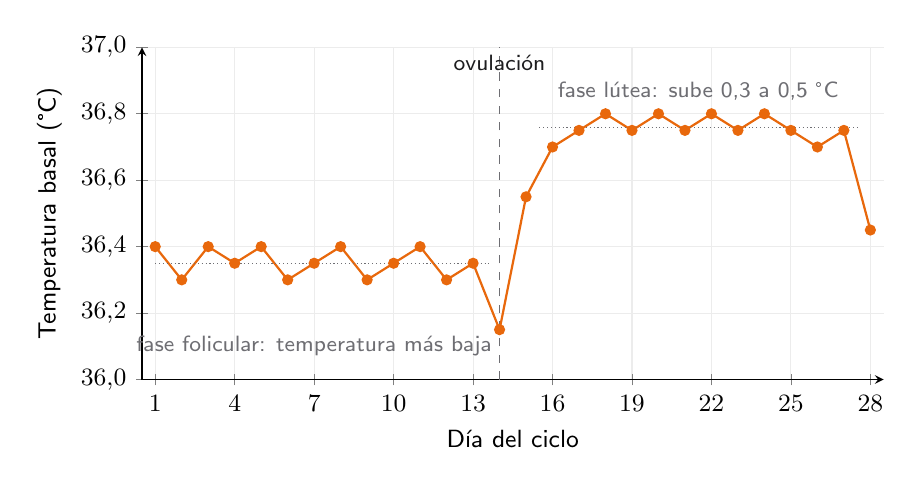
\begin{tikzpicture}[font=\small]
\begin{axis}[width=11cm,height=5.8cm,xmin=0.5,xmax=28.5,ymin=36.0,ymax=37.0,axis lines=left,xtick={1,4,...,28},
 ytick={36.0,36.2,...,37.0},yticklabel style={/pgf/number format/fixed,/pgf/number format/precision=1,/pgf/number format/fixed zerofill},
 xlabel={Día del ciclo},ylabel={Temperatura basal (°C)},grid=major,grid style={gray!15},clip=false]
\addplot[nar,thick,mark=*,mark size=1.6pt] coordinates {(1,36.4)(2,36.3)(3,36.4)(4,36.35)(5,36.4)(6,36.3)(7,36.35)(8,36.4)(9,36.3)(10,36.35)(11,36.4)(12,36.3)(13,36.35)(14,36.15)(15,36.55)(16,36.7)(17,36.75)(18,36.8)(19,36.75)(20,36.8)(21,36.75)(22,36.8)(23,36.75)(24,36.8)(25,36.75)(26,36.7)(27,36.75)(28,36.45)};
\draw[gris,dashed] (axis cs:14,36.0) -- (axis cs:14,37.0);
\node[anchor=south,font=\footnotesize,text=tinta] at (axis cs:14,36.9) {ovulación};
\draw[gris,densely dotted] (axis cs:1,36.35) -- (axis cs:13.6,36.35);
\node[font=\footnotesize,text=gris] at (axis cs:7,36.1) {fase folicular: temperatura más baja};
\draw[gris,densely dotted] (axis cs:15.5,36.76) -- (axis cs:27.5,36.76) node[midway,anchor=south,font=\footnotesize,text=gris,yshift=6pt] {fase lútea: sube 0,3 a 0,5 °C};
\end{axis}
\end{tikzpicture}
\end{document}
